% Options for packages loaded elsewhere
% Options for packages loaded elsewhere
\PassOptionsToPackage{unicode}{hyperref}
\PassOptionsToPackage{hyphens}{url}
\PassOptionsToPackage{dvipsnames,svgnames,x11names}{xcolor}
%
\documentclass[
  spanish,
  11pt,
  a4paper,
  DIV=11,
  numbers=noendperiod]{scrartcl}
\usepackage{xcolor}
\usepackage[margin=2.5cm]{geometry}
\usepackage{amsmath,amssymb}
\setcounter{secnumdepth}{5}
\usepackage{iftex}
\ifPDFTeX
  \usepackage[T1]{fontenc}
  \usepackage[utf8]{inputenc}
  \usepackage{textcomp} % provide euro and other symbols
\else % if luatex or xetex
  \usepackage{unicode-math} % this also loads fontspec
  \defaultfontfeatures{Scale=MatchLowercase}
  \defaultfontfeatures[\rmfamily]{Ligatures=TeX,Scale=1}
\fi
\usepackage{lmodern}
\ifPDFTeX\else
  % xetex/luatex font selection
  \setmainfont[]{Times New Roman}
\fi
% Use upquote if available, for straight quotes in verbatim environments
\IfFileExists{upquote.sty}{\usepackage{upquote}}{}
\IfFileExists{microtype.sty}{% use microtype if available
  \usepackage[]{microtype}
  \UseMicrotypeSet[protrusion]{basicmath} % disable protrusion for tt fonts
}{}
\makeatletter
\@ifundefined{KOMAClassName}{% if non-KOMA class
  \IfFileExists{parskip.sty}{%
    \usepackage{parskip}
  }{% else
    \setlength{\parindent}{0pt}
    \setlength{\parskip}{6pt plus 2pt minus 1pt}}
}{% if KOMA class
  \KOMAoptions{parskip=half}}
\makeatother
% Make \paragraph and \subparagraph free-standing
\makeatletter
\ifx\paragraph\undefined\else
  \let\oldparagraph\paragraph
  \renewcommand{\paragraph}{
    \@ifstar
      \xxxParagraphStar
      \xxxParagraphNoStar
  }
  \newcommand{\xxxParagraphStar}[1]{\oldparagraph*{#1}\mbox{}}
  \newcommand{\xxxParagraphNoStar}[1]{\oldparagraph{#1}\mbox{}}
\fi
\ifx\subparagraph\undefined\else
  \let\oldsubparagraph\subparagraph
  \renewcommand{\subparagraph}{
    \@ifstar
      \xxxSubParagraphStar
      \xxxSubParagraphNoStar
  }
  \newcommand{\xxxSubParagraphStar}[1]{\oldsubparagraph*{#1}\mbox{}}
  \newcommand{\xxxSubParagraphNoStar}[1]{\oldsubparagraph{#1}\mbox{}}
\fi
\makeatother

\usepackage{color}
\usepackage{fancyvrb}
\newcommand{\VerbBar}{|}
\newcommand{\VERB}{\Verb[commandchars=\\\{\}]}
\DefineVerbatimEnvironment{Highlighting}{Verbatim}{commandchars=\\\{\}}
% Add ',fontsize=\small' for more characters per line
\usepackage{framed}
\definecolor{shadecolor}{RGB}{241,243,245}
\newenvironment{Shaded}{\begin{snugshade}}{\end{snugshade}}
\newcommand{\AlertTok}[1]{\textcolor[rgb]{0.68,0.00,0.00}{#1}}
\newcommand{\AnnotationTok}[1]{\textcolor[rgb]{0.37,0.37,0.37}{#1}}
\newcommand{\AttributeTok}[1]{\textcolor[rgb]{0.40,0.45,0.13}{#1}}
\newcommand{\BaseNTok}[1]{\textcolor[rgb]{0.68,0.00,0.00}{#1}}
\newcommand{\BuiltInTok}[1]{\textcolor[rgb]{0.00,0.23,0.31}{#1}}
\newcommand{\CharTok}[1]{\textcolor[rgb]{0.13,0.47,0.30}{#1}}
\newcommand{\CommentTok}[1]{\textcolor[rgb]{0.37,0.37,0.37}{#1}}
\newcommand{\CommentVarTok}[1]{\textcolor[rgb]{0.37,0.37,0.37}{\textit{#1}}}
\newcommand{\ConstantTok}[1]{\textcolor[rgb]{0.56,0.35,0.01}{#1}}
\newcommand{\ControlFlowTok}[1]{\textcolor[rgb]{0.00,0.23,0.31}{\textbf{#1}}}
\newcommand{\DataTypeTok}[1]{\textcolor[rgb]{0.68,0.00,0.00}{#1}}
\newcommand{\DecValTok}[1]{\textcolor[rgb]{0.68,0.00,0.00}{#1}}
\newcommand{\DocumentationTok}[1]{\textcolor[rgb]{0.37,0.37,0.37}{\textit{#1}}}
\newcommand{\ErrorTok}[1]{\textcolor[rgb]{0.68,0.00,0.00}{#1}}
\newcommand{\ExtensionTok}[1]{\textcolor[rgb]{0.00,0.23,0.31}{#1}}
\newcommand{\FloatTok}[1]{\textcolor[rgb]{0.68,0.00,0.00}{#1}}
\newcommand{\FunctionTok}[1]{\textcolor[rgb]{0.28,0.35,0.67}{#1}}
\newcommand{\ImportTok}[1]{\textcolor[rgb]{0.00,0.46,0.62}{#1}}
\newcommand{\InformationTok}[1]{\textcolor[rgb]{0.37,0.37,0.37}{#1}}
\newcommand{\KeywordTok}[1]{\textcolor[rgb]{0.00,0.23,0.31}{\textbf{#1}}}
\newcommand{\NormalTok}[1]{\textcolor[rgb]{0.00,0.23,0.31}{#1}}
\newcommand{\OperatorTok}[1]{\textcolor[rgb]{0.37,0.37,0.37}{#1}}
\newcommand{\OtherTok}[1]{\textcolor[rgb]{0.00,0.23,0.31}{#1}}
\newcommand{\PreprocessorTok}[1]{\textcolor[rgb]{0.68,0.00,0.00}{#1}}
\newcommand{\RegionMarkerTok}[1]{\textcolor[rgb]{0.00,0.23,0.31}{#1}}
\newcommand{\SpecialCharTok}[1]{\textcolor[rgb]{0.37,0.37,0.37}{#1}}
\newcommand{\SpecialStringTok}[1]{\textcolor[rgb]{0.13,0.47,0.30}{#1}}
\newcommand{\StringTok}[1]{\textcolor[rgb]{0.13,0.47,0.30}{#1}}
\newcommand{\VariableTok}[1]{\textcolor[rgb]{0.07,0.07,0.07}{#1}}
\newcommand{\VerbatimStringTok}[1]{\textcolor[rgb]{0.13,0.47,0.30}{#1}}
\newcommand{\WarningTok}[1]{\textcolor[rgb]{0.37,0.37,0.37}{\textit{#1}}}

\usepackage{longtable,booktabs,array}
\usepackage{calc} % for calculating minipage widths
% Correct order of tables after \paragraph or \subparagraph
\usepackage{etoolbox}
\makeatletter
\patchcmd\longtable{\par}{\if@noskipsec\mbox{}\fi\par}{}{}
\makeatother
% Allow footnotes in longtable head/foot
\IfFileExists{footnotehyper.sty}{\usepackage{footnotehyper}}{\usepackage{footnote}}
\makesavenoteenv{longtable}
\usepackage{graphicx}
\makeatletter
\newsavebox\pandoc@box
\newcommand*\pandocbounded[1]{% scales image to fit in text height/width
  \sbox\pandoc@box{#1}%
  \Gscale@div\@tempa{\textheight}{\dimexpr\ht\pandoc@box+\dp\pandoc@box\relax}%
  \Gscale@div\@tempb{\linewidth}{\wd\pandoc@box}%
  \ifdim\@tempb\p@<\@tempa\p@\let\@tempa\@tempb\fi% select the smaller of both
  \ifdim\@tempa\p@<\p@\scalebox{\@tempa}{\usebox\pandoc@box}%
  \else\usebox{\pandoc@box}%
  \fi%
}
% Set default figure placement to htbp
\def\fps@figure{htbp}
\makeatother



\ifLuaTeX
\usepackage[bidi=basic]{babel}
\else
\usepackage[bidi=default]{babel}
\fi
\ifPDFTeX
\else
\babelfont{rm}[]{Times New Roman}
\fi
% get rid of language-specific shorthands (see #6817):
\let\LanguageShortHands\languageshorthands
\def\languageshorthands#1{}


\setlength{\emergencystretch}{3em} % prevent overfull lines

\providecommand{\tightlist}{%
  \setlength{\itemsep}{0pt}\setlength{\parskip}{0pt}}



 


\usepackage{booktabs}
\usepackage{longtable}
\usepackage{array}
\usepackage{multirow}
\usepackage{wrapfig}
\usepackage{float}
\usepackage{colortbl}
\usepackage{pdflscape}
\usepackage{tabu}
\usepackage{threeparttable}
\usepackage{threeparttablex}
\usepackage[normalem]{ulem}
\usepackage{makecell}
\usepackage{xcolor}
\KOMAoption{captions}{tableheading}
\makeatletter
\@ifpackageloaded{caption}{}{\usepackage{caption}}
\AtBeginDocument{%
\ifdefined\contentsname
  \renewcommand*\contentsname{Tabla de contenidos}
\else
  \newcommand\contentsname{Tabla de contenidos}
\fi
\ifdefined\listfigurename
  \renewcommand*\listfigurename{Listado de Figuras}
\else
  \newcommand\listfigurename{Listado de Figuras}
\fi
\ifdefined\listtablename
  \renewcommand*\listtablename{Listado de Tablas}
\else
  \newcommand\listtablename{Listado de Tablas}
\fi
\ifdefined\figurename
  \renewcommand*\figurename{Figura}
\else
  \newcommand\figurename{Figura}
\fi
\ifdefined\tablename
  \renewcommand*\tablename{Tabla}
\else
  \newcommand\tablename{Tabla}
\fi
}
\@ifpackageloaded{float}{}{\usepackage{float}}
\floatstyle{ruled}
\@ifundefined{c@chapter}{\newfloat{codelisting}{h}{lop}}{\newfloat{codelisting}{h}{lop}[chapter]}
\floatname{codelisting}{Listado}
\newcommand*\listoflistings{\listof{codelisting}{Listado de Listados}}
\makeatother
\makeatletter
\makeatother
\makeatletter
\@ifpackageloaded{caption}{}{\usepackage{caption}}
\@ifpackageloaded{subcaption}{}{\usepackage{subcaption}}
\makeatother
\usepackage{bookmark}
\IfFileExists{xurl.sty}{\usepackage{xurl}}{} % add URL line breaks if available
\urlstyle{same}
\hypersetup{
  pdftitle={Índices ecológicos},
  pdfauthor={Santos G},
  pdflang={es},
  colorlinks=true,
  linkcolor={blue},
  filecolor={Maroon},
  citecolor={Blue},
  urlcolor={Blue},
  pdfcreator={LaTeX via pandoc}}


\title{Índices ecológicos}
\author{Santos G}
\date{}
\begin{document}
\maketitle

\renewcommand*\contentsname{Tabla de contenidos}
{
\hypersetup{linkcolor=}
\setcounter{tocdepth}{2}
\tableofcontents
}

\section{Contexto del proyecto}\label{contexto-del-proyecto}

El presente documento guía describe el dataset palmerpenguins
(mediciones morfométricas y metadatos de tres especies de pingüinos:
\emph{Adelie}, \emph{Chinstrap} y \emph{Gentoo}). Antes de calcular
índices ecológicos o métricas de biodiversidad, es fundamental evaluar
la calidad y consistencia de los datos. Para ello se realizará la
limpieza y revisión inicial de los datos (nombres, estructura, NA,
duplicados, categorías).

\section{Limpieza y revisión inicial de los
datos}\label{limpieza-y-revisiuxf3n-inicial-de-los-datos}

\begin{Shaded}
\begin{Highlighting}[numbers=left,,]
\CommentTok{\#|label: prep}
\CommentTok{\#Librerías}
\FunctionTok{library}\NormalTok{(tidyverse)}
\FunctionTok{library}\NormalTok{(janitor)}
\FunctionTok{library}\NormalTok{(skimr)}
\FunctionTok{library}\NormalTok{(palmerpenguins)}

\NormalTok{df\_raw }\OtherTok{\textless{}{-}}\NormalTok{ penguins }\SpecialCharTok{\%\textgreater{}\%} \FunctionTok{as\_tibble}\NormalTok{() }\CommentTok{\# guardo raw para auditoría}
\end{Highlighting}
\end{Shaded}

\begin{Shaded}
\begin{Highlighting}[numbers=left,,]
\CommentTok{\#|label: clean\_names}
\NormalTok{df }\OtherTok{\textless{}{-}}\NormalTok{ df\_raw }\SpecialCharTok{\%\textgreater{}\%} \FunctionTok{clean\_names}\NormalTok{()}
\FunctionTok{names}\NormalTok{(df) }\CommentTok{\# comprobar}
\end{Highlighting}
\end{Shaded}

\begin{verbatim}
[1] "species"           "island"            "bill_length_mm"   
[4] "bill_depth_mm"     "flipper_length_mm" "body_mass_g"      
[7] "sex"               "year"             
\end{verbatim}

\begin{Shaded}
\begin{Highlighting}[numbers=left,,]
\CommentTok{\#|label: skim}
\FunctionTok{skim}\NormalTok{(df) }\CommentTok{\#Resumen rápido (estructura + NA)}
\end{Highlighting}
\end{Shaded}

\begin{longtable}[]{@{}ll@{}}
\caption{Data summary}\tabularnewline
\toprule\noalign{}
\endfirsthead
\endhead
\bottomrule\noalign{}
\endlastfoot
Name & df \\
Number of rows & 344 \\
Number of columns & 8 \\
\_\_\_\_\_\_\_\_\_\_\_\_\_\_\_\_\_\_\_\_\_\_\_ & \\
Column type frequency: & \\
factor & 3 \\
numeric & 5 \\
\_\_\_\_\_\_\_\_\_\_\_\_\_\_\_\_\_\_\_\_\_\_\_\_ & \\
Group variables & None \\
\end{longtable}

\textbf{Variable type: factor}

\begin{longtable}[]{@{}
  >{\raggedright\arraybackslash}p{(\linewidth - 10\tabcolsep) * \real{0.1687}}
  >{\raggedleft\arraybackslash}p{(\linewidth - 10\tabcolsep) * \real{0.1205}}
  >{\raggedleft\arraybackslash}p{(\linewidth - 10\tabcolsep) * \real{0.1687}}
  >{\raggedright\arraybackslash}p{(\linewidth - 10\tabcolsep) * \real{0.0964}}
  >{\raggedleft\arraybackslash}p{(\linewidth - 10\tabcolsep) * \real{0.1084}}
  >{\raggedright\arraybackslash}p{(\linewidth - 10\tabcolsep) * \real{0.3373}}@{}}
\toprule\noalign{}
\begin{minipage}[b]{\linewidth}\raggedright
skim\_variable
\end{minipage} & \begin{minipage}[b]{\linewidth}\raggedleft
n\_missing
\end{minipage} & \begin{minipage}[b]{\linewidth}\raggedleft
complete\_rate
\end{minipage} & \begin{minipage}[b]{\linewidth}\raggedright
ordered
\end{minipage} & \begin{minipage}[b]{\linewidth}\raggedleft
n\_unique
\end{minipage} & \begin{minipage}[b]{\linewidth}\raggedright
top\_counts
\end{minipage} \\
\midrule\noalign{}
\endhead
\bottomrule\noalign{}
\endlastfoot
species & 0 & 1.00 & FALSE & 3 & Ade: 152, Gen: 124, Chi: 68 \\
island & 0 & 1.00 & FALSE & 3 & Bis: 168, Dre: 124, Tor: 52 \\
sex & 11 & 0.97 & FALSE & 2 & mal: 168, fem: 165 \\
\end{longtable}

\textbf{Variable type: numeric}

\begin{longtable}[]{@{}
  >{\raggedright\arraybackslash}p{(\linewidth - 20\tabcolsep) * \real{0.1800}}
  >{\raggedleft\arraybackslash}p{(\linewidth - 20\tabcolsep) * \real{0.1000}}
  >{\raggedleft\arraybackslash}p{(\linewidth - 20\tabcolsep) * \real{0.1400}}
  >{\raggedleft\arraybackslash}p{(\linewidth - 20\tabcolsep) * \real{0.0800}}
  >{\raggedleft\arraybackslash}p{(\linewidth - 20\tabcolsep) * \real{0.0700}}
  >{\raggedleft\arraybackslash}p{(\linewidth - 20\tabcolsep) * \real{0.0700}}
  >{\raggedleft\arraybackslash}p{(\linewidth - 20\tabcolsep) * \real{0.0800}}
  >{\raggedleft\arraybackslash}p{(\linewidth - 20\tabcolsep) * \real{0.0800}}
  >{\raggedleft\arraybackslash}p{(\linewidth - 20\tabcolsep) * \real{0.0700}}
  >{\raggedleft\arraybackslash}p{(\linewidth - 20\tabcolsep) * \real{0.0700}}
  >{\raggedright\arraybackslash}p{(\linewidth - 20\tabcolsep) * \real{0.0600}}@{}}
\toprule\noalign{}
\begin{minipage}[b]{\linewidth}\raggedright
skim\_variable
\end{minipage} & \begin{minipage}[b]{\linewidth}\raggedleft
n\_missing
\end{minipage} & \begin{minipage}[b]{\linewidth}\raggedleft
complete\_rate
\end{minipage} & \begin{minipage}[b]{\linewidth}\raggedleft
mean
\end{minipage} & \begin{minipage}[b]{\linewidth}\raggedleft
sd
\end{minipage} & \begin{minipage}[b]{\linewidth}\raggedleft
p0
\end{minipage} & \begin{minipage}[b]{\linewidth}\raggedleft
p25
\end{minipage} & \begin{minipage}[b]{\linewidth}\raggedleft
p50
\end{minipage} & \begin{minipage}[b]{\linewidth}\raggedleft
p75
\end{minipage} & \begin{minipage}[b]{\linewidth}\raggedleft
p100
\end{minipage} & \begin{minipage}[b]{\linewidth}\raggedright
hist
\end{minipage} \\
\midrule\noalign{}
\endhead
\bottomrule\noalign{}
\endlastfoot
bill\_length\_mm & 2 & 0.99 & 43.92 & 5.46 & 32.1 & 39.23 & 44.45 & 48.5
& 59.6 & ▃▇▇▆▁ \\
bill\_depth\_mm & 2 & 0.99 & 17.15 & 1.97 & 13.1 & 15.60 & 17.30 & 18.7
& 21.5 & ▅▅▇▇▂ \\
flipper\_length\_mm & 2 & 0.99 & 200.92 & 14.06 & 172.0 & 190.00 &
197.00 & 213.0 & 231.0 & ▂▇▃▅▂ \\
body\_mass\_g & 2 & 0.99 & 4201.75 & 801.95 & 2700.0 & 3550.00 & 4050.00
& 4750.0 & 6300.0 & ▃▇▆▃▂ \\
year & 0 & 1.00 & 2008.03 & 0.82 & 2007.0 & 2007.00 & 2008.00 & 2009.0 &
2009.0 & ▇▁▇▁▇ \\
\end{longtable}

De acuerdo con la \textbf{Tabla 1}, la base de datos \texttt{penguins}
contiene 344 registros y 8 variables, de las cuales 3 son categóricas
(\texttt{species}, \texttt{island}, \texttt{sex}) y 5 numéricas
(\texttt{bill\_length\_mm}, \texttt{bill\_depth\_mm},
\texttt{flipper\_length\_mm}, \texttt{body\_mass\_g}, \texttt{year}).

En las variables categóricas:

\begin{itemize}
\item
  \texttt{species}: tres categorías (\emph{Adelie} = 152, \emph{Gentoo}
  = 124, \emph{Chinstrap} = 68), sin valores faltantes.
\item
  \texttt{island}: tres categorías (\emph{Biscoe} = 168, \emph{Dream} =
  124, \emph{Torgersen} = 52), sin valores faltantes.
\item
  \texttt{sex}: dos categorías (\emph{male} = 168, \emph{female} = 165)
  con 11 valores faltantes (3\%).
\end{itemize}

En las variables numéricas:

\begin{itemize}
\item
  \texttt{bill\_length\_mm}: media ≈ 43.9 mm, rango 32.1--59.6 mm, con 2
  valores faltantes.
\item
  \texttt{bill\_depth\_mm}: media ≈ 17.2 mm, rango 13.1--21.5 mm, con 2
  faltantes.
\item
  \texttt{flipper\_length\_mm}: media ≈ 200.9 mm, rango 172--231 mm, con
  2 faltantes.
\item
  \texttt{body\_mass\_g}: media ≈ 4201 g, rango 2700--6300 g, con 2
  faltantes.
\item
  \texttt{year}: muestreos entre 2007--2009, sin valores faltantes.
\end{itemize}

\textbf{Interpretación general:}

\begin{itemize}
\item
  Los nombres de variables ya están estandarizados.
\item
  El dataset presenta un bajo porcentaje de NA (\textless1\% en
  mediciones y 3\% en \texttt{sex}). Estos casos podrán eliminarse o
  imputarse según el análisis.
\item
  No se observan inconsistencias de escritura en categorías ni rangos
  numéricos irreales.
\end{itemize}

\begin{Shaded}
\begin{Highlighting}[numbers=left,,]
\CommentTok{\#|label: duplicates}
\NormalTok{n\_dup }\OtherTok{\textless{}{-}} \FunctionTok{sum}\NormalTok{(}\FunctionTok{duplicated}\NormalTok{(df))}
\NormalTok{n\_dup }\CommentTok{\# Número de filas duplicadas}
\end{Highlighting}
\end{Shaded}

\begin{verbatim}
[1] 0
\end{verbatim}

\begin{Shaded}
\begin{Highlighting}[numbers=left,,]
\CommentTok{\# si quieres, ver filas duplicadas (opcional)}
\NormalTok{df }\SpecialCharTok{\%\textgreater{}\%} \FunctionTok{filter}\NormalTok{(}\FunctionTok{duplicated}\NormalTok{(.)) }\SpecialCharTok{\%\textgreater{}\%} \FunctionTok{head}\NormalTok{()}
\end{Highlighting}
\end{Shaded}

\begin{verbatim}
# A tibble: 0 x 8
# i 8 variables: species <fct>, island <fct>, bill_length_mm <dbl>,
#   bill_depth_mm <dbl>, flipper_length_mm <int>, body_mass_g <int>, sex <fct>,
#   year <int>
\end{verbatim}

\begin{Shaded}
\begin{Highlighting}[numbers=left,,]
\CommentTok{\# eliminar duplicados exactos (opcional)}
\NormalTok{df }\OtherTok{\textless{}{-}}\NormalTok{ df }\SpecialCharTok{\%\textgreater{}\%} \FunctionTok{distinct}\NormalTok{()}
\end{Highlighting}
\end{Shaded}

En este caso no se encontraron filas duplicadas (\texttt{n\_dup\ =\ 0}).

\textbf{Interpretación general:}

\begin{itemize}
\item
  Cuando no hay duplicados, no se requieren cambios.
\item
  Si en futuros proyectos aparecen duplicados, se recomienda, verificar
  primero si son errores de registro o réplicas biológicas válidas, ya
  que si son errores (mismo individuo registrado más de una vez), deben
  eliminarse, caso contrario deben mantenerse o promediarse según el
  objetivo del estudio.
\end{itemize}

\begin{Shaded}
\begin{Highlighting}[numbers=left,,]
\CommentTok{\#Variables categóricas}
\NormalTok{df }\SpecialCharTok{\%\textgreater{}\%} \FunctionTok{summarise}\NormalTok{(}\FunctionTok{across}\NormalTok{(}\FunctionTok{where}\NormalTok{(is.character), n\_distinct))}
\end{Highlighting}
\end{Shaded}

\begin{verbatim}
# A tibble: 1 x 0
\end{verbatim}

\begin{Shaded}
\begin{Highlighting}[numbers=left,,]
\NormalTok{df }\SpecialCharTok{\%\textgreater{}\%} \FunctionTok{summarise}\NormalTok{(}\FunctionTok{across}\NormalTok{(}\FunctionTok{where}\NormalTok{(is.factor), n\_distinct))}
\end{Highlighting}
\end{Shaded}

\begin{verbatim}
# A tibble: 1 x 3
  species island   sex
    <int>  <int> <int>
1       3      3     3
\end{verbatim}

\begin{Shaded}
\begin{Highlighting}[numbers=left,,]
\NormalTok{df }\SpecialCharTok{\%\textgreater{}\%} \FunctionTok{count}\NormalTok{(species)}
\end{Highlighting}
\end{Shaded}

\begin{verbatim}
# A tibble: 3 x 2
  species       n
  <fct>     <int>
1 Adelie      152
2 Chinstrap    68
3 Gentoo      124
\end{verbatim}

\begin{Shaded}
\begin{Highlighting}[numbers=left,,]
\NormalTok{df }\SpecialCharTok{\%\textgreater{}\%} \FunctionTok{count}\NormalTok{(island)}
\end{Highlighting}
\end{Shaded}

\begin{verbatim}
# A tibble: 3 x 2
  island        n
  <fct>     <int>
1 Biscoe      168
2 Dream       124
3 Torgersen    52
\end{verbatim}

\begin{Shaded}
\begin{Highlighting}[numbers=left,,]
\NormalTok{df }\SpecialCharTok{\%\textgreater{}\%} \FunctionTok{count}\NormalTok{(sex)}
\end{Highlighting}
\end{Shaded}

\begin{verbatim}
# A tibble: 3 x 2
  sex        n
  <fct>  <int>
1 female   165
2 male     168
3 <NA>      11
\end{verbatim}

\begin{Shaded}
\begin{Highlighting}[numbers=left,,]
\CommentTok{\#Tipos de variables (convertir a factor si hace falta)}
\NormalTok{df }\OtherTok{\textless{}{-}}\NormalTok{ df }\SpecialCharTok{\%\textgreater{}\%} 
  \FunctionTok{mutate}\NormalTok{(}\AttributeTok{species =} \FunctionTok{as.factor}\NormalTok{(species),}
         \AttributeTok{island  =} \FunctionTok{as.factor}\NormalTok{(island),}
         \AttributeTok{sex     =} \FunctionTok{as.factor}\NormalTok{(sex))}

\CommentTok{\#Revisar posibles inconsistencias de texto}
\FunctionTok{unique}\NormalTok{(df}\SpecialCharTok{$}\NormalTok{species)}
\end{Highlighting}
\end{Shaded}

\begin{verbatim}
[1] Adelie    Gentoo    Chinstrap
Levels: Adelie Chinstrap Gentoo
\end{verbatim}

\begin{Shaded}
\begin{Highlighting}[numbers=left,,]
\FunctionTok{unique}\NormalTok{(df}\SpecialCharTok{$}\NormalTok{island)}
\end{Highlighting}
\end{Shaded}

\begin{verbatim}
[1] Torgersen Biscoe    Dream    
Levels: Biscoe Dream Torgersen
\end{verbatim}

\begin{Shaded}
\begin{Highlighting}[numbers=left,,]
\FunctionTok{unique}\NormalTok{(df}\SpecialCharTok{$}\NormalTok{sex)}
\end{Highlighting}
\end{Shaded}

\begin{verbatim}
[1] male   female <NA>  
Levels: female male
\end{verbatim}

\begin{Shaded}
\begin{Highlighting}[numbers=left,,]
\NormalTok{df1 }\OtherTok{\textless{}{-}}\NormalTok{ df }\SpecialCharTok{\%\textgreater{}\%} \FunctionTok{select}\NormalTok{(}\SpecialCharTok{{-}}\NormalTok{year) }\CommentTok{\#Eliminar columnas innecesarias}
\end{Highlighting}
\end{Shaded}

Las variables categóricas (\texttt{species}, \texttt{island},
\texttt{sex}) presentan 3, 3 y 2 categorías respectivamente, sin
inconsistencias de escritura. Se ajustaron los tipos de variable a
\texttt{factor} y se eliminó la columna \texttt{year}, ya que no será
utilizada en los análisis posteriores.

\begin{Shaded}
\begin{Highlighting}[numbers=left,,]
\CommentTok{\# Boxplots rápidos para ver rangos y "outliers" visuales}
\NormalTok{key\_vars }\OtherTok{\textless{}{-}} \FunctionTok{c}\NormalTok{(}\StringTok{"bill\_length\_mm"}\NormalTok{,}\StringTok{"bill\_depth\_mm"}\NormalTok{,}\StringTok{"flipper\_length\_mm"}\NormalTok{,}
              \StringTok{"body\_mass\_g"}\NormalTok{)}

\NormalTok{df }\SpecialCharTok{\%\textgreater{}\%}
  \FunctionTok{select}\NormalTok{(}\FunctionTok{all\_of}\NormalTok{(key\_vars)) }\SpecialCharTok{\%\textgreater{}\%}
  \FunctionTok{pivot\_longer}\NormalTok{(}\FunctionTok{everything}\NormalTok{(), }\AttributeTok{names\_to =} \StringTok{"variable"}\NormalTok{, }\AttributeTok{values\_to =} \StringTok{"value"}\NormalTok{) }\SpecialCharTok{\%\textgreater{}\%}
  \FunctionTok{ggplot}\NormalTok{(}\FunctionTok{aes}\NormalTok{(}\AttributeTok{x =}\NormalTok{ variable, }\AttributeTok{y =}\NormalTok{ value)) }\SpecialCharTok{+}
  \FunctionTok{geom\_boxplot}\NormalTok{() }\SpecialCharTok{+}
  \FunctionTok{coord\_flip}\NormalTok{() }\SpecialCharTok{+}
  \FunctionTok{labs}\NormalTok{(}\AttributeTok{title =} \StringTok{"Boxplots rápidos: rangos y valores extremos"}\NormalTok{,}
       \AttributeTok{x =} \StringTok{""}\NormalTok{, }\AttributeTok{y =} \StringTok{"Valor"}\NormalTok{) }\SpecialCharTok{+}
  \FunctionTok{theme\_minimal}\NormalTok{(}\AttributeTok{base\_size =} \DecValTok{13}\NormalTok{) }\SpecialCharTok{+}
  \FunctionTok{theme}\NormalTok{(}
   \AttributeTok{plot.title =} \FunctionTok{element\_text}\NormalTok{(}\AttributeTok{hjust =} \FloatTok{0.5}\NormalTok{, }\AttributeTok{face =} \StringTok{"bold"}\NormalTok{),}
   \AttributeTok{legend.position =} \StringTok{"none"}\NormalTok{,}
   \AttributeTok{strip.text =} \FunctionTok{element\_text}\NormalTok{(}\AttributeTok{face =} \StringTok{"bold"}\NormalTok{)}
\NormalTok{   )}
\end{Highlighting}
\end{Shaded}

\begin{figure}[H]

{\centering \pandocbounded{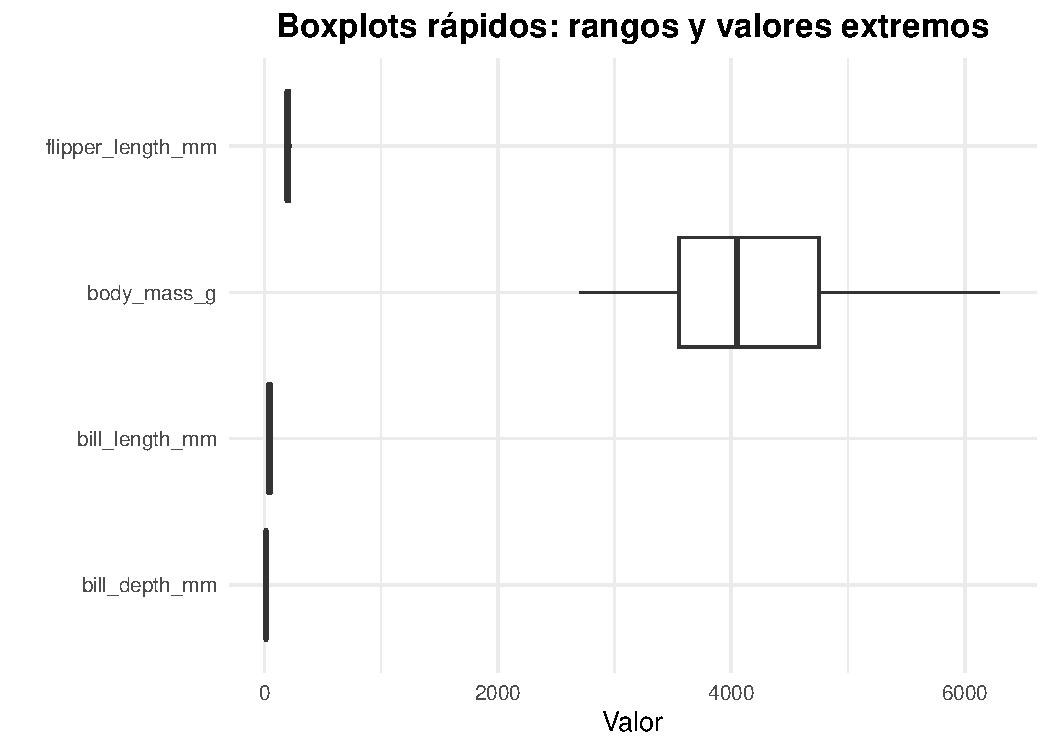
\includegraphics[keepaspectratio]{Índices-ecológicos_files/figure-pdf/ranges_boxplot variables númericas-1.pdf}}

}

\caption{Rangos y valores extremos de variables morfométricas.}

\end{figure}%

En la \textbf{Figura 1}, se observa que los rangos numéricos se
encuentran dentro de lo esperado para las especies registradas, y los
gráficos de caja confirman que los valores extremos corresponden a
variabilidad natural más que a errores de registro.

\begin{Shaded}
\begin{Highlighting}[numbers=left,,]
\CommentTok{\#|label: Manejo de los NA}

\CommentTok{\# Manejo de los NA}
\NormalTok{df }\OtherTok{\textless{}{-}}\NormalTok{ df }\SpecialCharTok{\%\textgreater{}\%}
  \FunctionTok{mutate}\NormalTok{(}
    \AttributeTok{n\_na\_numeric =} \FunctionTok{rowSums}\NormalTok{(}\FunctionTok{is.na}\NormalTok{(}\FunctionTok{select}\NormalTok{(., bill\_length\_mm, bill\_depth\_mm,}
\NormalTok{                                        flipper\_length\_mm, body\_mass\_g)))}
\NormalTok{  )}

\NormalTok{df }\OtherTok{\textless{}{-}}\NormalTok{ df }\SpecialCharTok{\%\textgreater{}\%}
  \FunctionTok{mutate}\NormalTok{(}
    \AttributeTok{sex =} \FunctionTok{case\_when}\NormalTok{(}
      \FunctionTok{is.na}\NormalTok{(sex) }\SpecialCharTok{\&}\NormalTok{ n\_na\_numeric }\SpecialCharTok{\textless{}=} \DecValTok{1} \SpecialCharTok{\textasciitilde{}} \StringTok{"Unknown"}\NormalTok{,  }\CommentTok{\# casi toda la info presente}
      \ConstantTok{TRUE} \SpecialCharTok{\textasciitilde{}} \FunctionTok{as.character}\NormalTok{(sex)                    }\CommentTok{\# dejar como está}
\NormalTok{    )}
\NormalTok{  )}

\NormalTok{df }\OtherTok{\textless{}{-}}\NormalTok{ df }\SpecialCharTok{\%\textgreater{}\%}
  \FunctionTok{filter}\NormalTok{(}\SpecialCharTok{!}\NormalTok{(}\FunctionTok{is.na}\NormalTok{(bill\_length\_mm) }\SpecialCharTok{\&}
           \FunctionTok{is.na}\NormalTok{(bill\_depth\_mm) }\SpecialCharTok{\&}
           \FunctionTok{is.na}\NormalTok{(flipper\_length\_mm) }\SpecialCharTok{\&}
           \FunctionTok{is.na}\NormalTok{(body\_mass\_g)))}


\NormalTok{df }\OtherTok{\textless{}{-}}\NormalTok{ df }\SpecialCharTok{\%\textgreater{}\%} \FunctionTok{select}\NormalTok{(}\SpecialCharTok{{-}}\NormalTok{n\_na\_numeric) }\CommentTok{\#Eliminar columnas innecesarias}
\end{Highlighting}
\end{Shaded}

Se contabilizó cuántas mediciones morfométricas tiene cada registro
(bill\_length\_mm, bill\_depth\_mm, flipper\_length\_mm, body\_mass\_g).

\begin{itemize}
\item
  Registros con ≥ 3 mediciones y sex = NA fueron etiquetados como sex =
  ``Unknown'': son registros con información morfométrica suficiente
  como para conservarlos en análisis de biodiversidad/morfometría, pero
  sin identificación sexual.
\item
  Registros con 0 mediciones (probablemente avistamientos sin
  mediciones) fueron eliminados, ya que no aportan datos morfométricos
  para los análisis previstos.
\end{itemize}

\section{Construcción de la matriz de
abundancia}\label{construcciuxf3n-de-la-matriz-de-abundancia}

\begin{Shaded}
\begin{Highlighting}[numbers=left,,]
\CommentTok{\#Librerías}
\FunctionTok{library}\NormalTok{(knitr)}
\FunctionTok{library}\NormalTok{(kableExtra)}
\end{Highlighting}
\end{Shaded}

\begin{Shaded}
\begin{Highlighting}[numbers=left,,]
\CommentTok{\# Matriz especie x isla}
\NormalTok{abund }\OtherTok{\textless{}{-}}\NormalTok{ df }\SpecialCharTok{\%\textgreater{}\%}
  \FunctionTok{count}\NormalTok{(island, species) }\SpecialCharTok{\%\textgreater{}\%}
  \FunctionTok{pivot\_wider}\NormalTok{(}\AttributeTok{names\_from =}\NormalTok{ species, }\AttributeTok{values\_from =}\NormalTok{ n, }\AttributeTok{values\_fill =} \DecValTok{0}\NormalTok{)}

\CommentTok{\# Crear tabla}
\NormalTok{abund }\SpecialCharTok{\%\textgreater{}\%}
  \FunctionTok{kable}\NormalTok{(}\AttributeTok{caption =} \StringTok{"Abundancia de pingüinos por especie e isla }
\StringTok{        en el archipiélago Palmer."}\NormalTok{,}
        \AttributeTok{align =} \StringTok{"lccc"}\NormalTok{,}
        \AttributeTok{col.names =} \FunctionTok{c}\NormalTok{(}\StringTok{"Isla"}\NormalTok{, }\StringTok{"Adelie"}\NormalTok{, }\StringTok{"Gentoo"}\NormalTok{, }\StringTok{"Chinstrap"}\NormalTok{)) }\SpecialCharTok{\%\textgreater{}\%}
  \FunctionTok{kable\_styling}\NormalTok{(}\AttributeTok{full\_width =} \ConstantTok{FALSE}\NormalTok{, }\AttributeTok{bootstrap\_options =} \FunctionTok{c}\NormalTok{(}\StringTok{"striped"}\NormalTok{, }
      \StringTok{"hover"}\NormalTok{, }\StringTok{"condensed"}\NormalTok{))}
\end{Highlighting}
\end{Shaded}

\begin{longtable}[t]{lccc}
\caption{\label{tab:abundancia}Abundancia de pingüinos por especie e isla 
        en el archipiélago Palmer.}\\
\toprule
Isla & Adelie & Gentoo & Chinstrap\\
\midrule
Biscoe & 44 & 123 & 0\\
Dream & 56 & 0 & 68\\
Torgersen & 51 & 0 & 0\\
\bottomrule
\end{longtable}

Aunque \texttt{palmerpenguins} no es un dataset clásico de abundancias
de especies (es más bien morfométrico), podemos adaptarlo, para ello
tomamos las especies como categorías biológicas (3 especies:
\emph{Adelie}, \emph{Gentoo}, \emph{Chinstrap}) y contamos número de
individuos por especie y por isla, para tener una matriz de abundancias
que nos permita calcular índices de biodiversidad.

En la \textbf{Tabla 4} se muestra la distribución de individuos por
especie e isla:

\begin{itemize}
\item
  \textbf{Biscoe}: domina la especie \emph{Gentoo} con 123 individuos,
  seguida por \emph{Adelie} con 44. No se registran individuos en
  \emph{Chinstrap}.
\item
  \textbf{Dream}: comunidad más equilibrada, con 56 \emph{Adelie} y 68
  \emph{Chinstrap}. No se registran individuos en \emph{Gentoo}.
\item
  \textbf{Torgersen}: exclusiva de \emph{Adelie}, con 51 individuos; no
  se observan individuos de \emph{Gentoo} ni \emph{Chinstrap}.
\end{itemize}

\textbf{Interpretación general:} Cada isla presenta una composición
particular. Mientras Biscoe está claramente dominada por \emph{Gentoo},
Dream muestra coexistencia entre \emph{Adelie} y \emph{Chinstrap}, y
Torgersen resulta la más restringida, con presencia exclusiva de
\emph{Adelie}. Esta variación espacial será clave al analizar los
índices de diversidad y equidad.

\section{Calcular índices de diversidad y curvas de
rarefacción}\label{calcular-uxedndices-de-diversidad-y-curvas-de-rarefacciuxf3n}

\begin{Shaded}
\begin{Highlighting}[numbers=left,,]
\CommentTok{\#Librerías}
\FunctionTok{library}\NormalTok{(vegan)}
\end{Highlighting}
\end{Shaded}

\begin{Shaded}
\begin{Highlighting}[numbers=left,,]
\CommentTok{\# Matriz especie x isla}
\NormalTok{mat }\OtherTok{\textless{}{-}}\NormalTok{ abund }\SpecialCharTok{\%\textgreater{}\%} \FunctionTok{select}\NormalTok{(}\SpecialCharTok{{-}}\NormalTok{island) }\SpecialCharTok{\%\textgreater{}\%} \FunctionTok{as.matrix}\NormalTok{()}
\FunctionTok{rownames}\NormalTok{(mat) }\OtherTok{\textless{}{-}}\NormalTok{ abund}\SpecialCharTok{$}\NormalTok{island}

\CommentTok{\# índices}
\NormalTok{shannon  }\OtherTok{\textless{}{-}} \FunctionTok{diversity}\NormalTok{(mat, }\AttributeTok{index =} \StringTok{"shannon"}\NormalTok{)}
\NormalTok{simpson  }\OtherTok{\textless{}{-}} \FunctionTok{diversity}\NormalTok{(mat, }\AttributeTok{index =} \StringTok{"simpson"}\NormalTok{)}
\NormalTok{richness }\OtherTok{\textless{}{-}} \FunctionTok{specnumber}\NormalTok{(mat)}
\NormalTok{evenness }\OtherTok{\textless{}{-}} \FunctionTok{ifelse}\NormalTok{(richness }\SpecialCharTok{\textgreater{}} \DecValTok{1}\NormalTok{, shannon }\SpecialCharTok{/} \FunctionTok{log}\NormalTok{(richness), }\DecValTok{0}\NormalTok{) }\CommentTok{\# corregido}

\NormalTok{indices }\OtherTok{\textless{}{-}} \FunctionTok{data.frame}\NormalTok{(}
  \AttributeTok{Isla     =} \FunctionTok{rownames}\NormalTok{(mat),}
  \AttributeTok{Riqueza  =}\NormalTok{ richness,}
  \AttributeTok{Shannon  =} \FunctionTok{round}\NormalTok{(shannon, }\DecValTok{2}\NormalTok{),}
  \AttributeTok{Simpson  =} \FunctionTok{round}\NormalTok{(simpson, }\DecValTok{2}\NormalTok{),}
  \AttributeTok{Equidad  =} \FunctionTok{round}\NormalTok{(evenness, }\DecValTok{2}\NormalTok{)}
\NormalTok{)}

\NormalTok{knitr}\SpecialCharTok{::}\FunctionTok{kable}\NormalTok{(indices, }\AttributeTok{caption =} \ConstantTok{NULL}\NormalTok{)}
\end{Highlighting}
\end{Shaded}

\begin{longtable}[]{@{}llrrrr@{}}
\caption{Índices de diversidad de especies de pingüinos por
isla.}\tabularnewline
\toprule\noalign{}
& Isla & Riqueza & Shannon & Simpson & Equidad \\
\midrule\noalign{}
\endfirsthead
\toprule\noalign{}
& Isla & Riqueza & Shannon & Simpson & Equidad \\
\midrule\noalign{}
\endhead
\bottomrule\noalign{}
\endlastfoot
Biscoe & Biscoe & 2 & 0.58 & 0.39 & 0.83 \\
Dream & Dream & 2 & 0.69 & 0.50 & 0.99 \\
Torgersen & Torgersen & 1 & 0.00 & 0.00 & 0.00 \\
\end{longtable}

\begin{Shaded}
\begin{Highlighting}[numbers=left,,]
\CommentTok{\# Curvas de rarefacción}
\FunctionTok{rarecurve}\NormalTok{(mat, }\AttributeTok{step =} \DecValTok{10}\NormalTok{, }\AttributeTok{sample =} \FunctionTok{min}\NormalTok{(}\FunctionTok{rowSums}\NormalTok{(mat)), }\AttributeTok{col =} \DecValTok{1}\SpecialCharTok{:}\DecValTok{3}\NormalTok{, }
          \AttributeTok{lwd =} \DecValTok{2}\NormalTok{, }\AttributeTok{ylab =} \StringTok{"Riqueza de especies"}\NormalTok{)}
\FunctionTok{legend}\NormalTok{(}\StringTok{"bottomright"}\NormalTok{, }\AttributeTok{legend =} \FunctionTok{rownames}\NormalTok{(mat), }\AttributeTok{col =} \DecValTok{1}\SpecialCharTok{:}\DecValTok{3}\NormalTok{, }
       \AttributeTok{lwd =} \DecValTok{2}\NormalTok{, }\AttributeTok{bty =} \StringTok{"n"}\NormalTok{)}
\end{Highlighting}
\end{Shaded}

\begin{figure}[H]

{\centering \pandocbounded{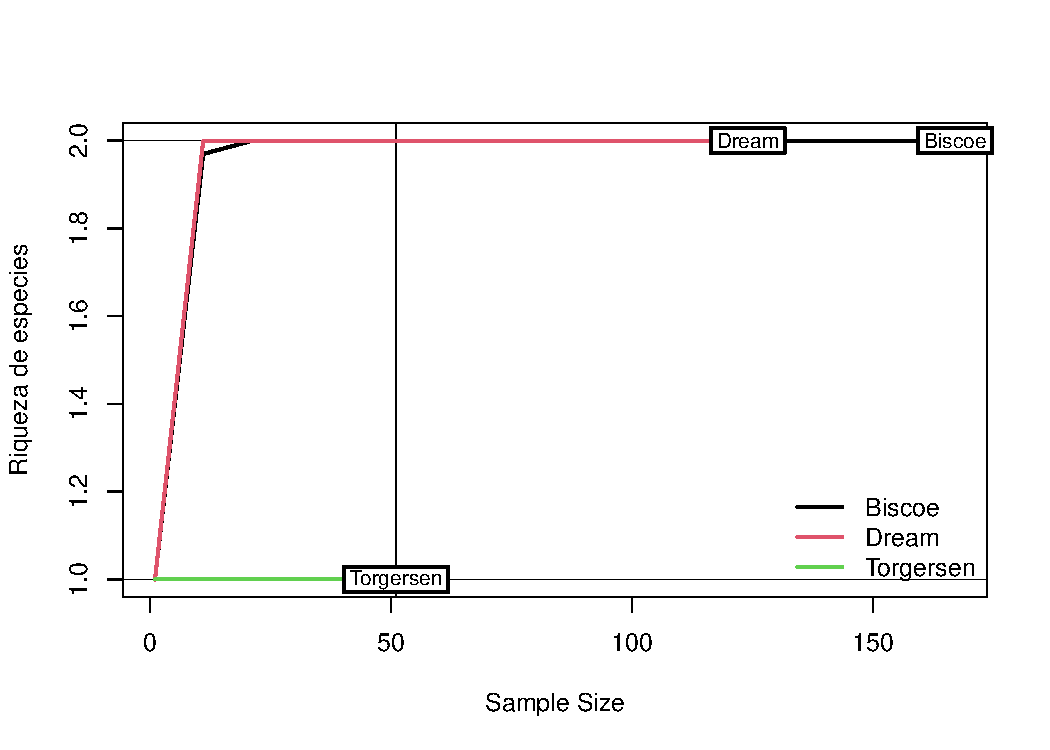
\includegraphics[keepaspectratio]{Índices-ecológicos_files/figure-pdf/rarefaccion-1.pdf}}

}

\caption{Curvas de rarefacción de riqueza de especies de pingüinos por
isla.}

\end{figure}%




\end{document}
